
\documentclass[a4paper,12pt]{report}
%    \renewcommand{\baselinestretch}{1.6}      % interline spacing
%
% \includeonly{}
%
%			PREAMBOLO
%
\usepackage[a4paper]{geometry}
\usepackage{amssymb,amsmath,amsthm}
\usepackage{graphicx}
\usepackage{url}
\usepackage{hyperref}
\usepackage{epsfig}
\usepackage[italian, english]{babel}
\usepackage{setspace}
\usepackage{style}
\graphicspath{ {./img/} }
\usepackage{float}
\usepackage{booktabs}


% per le accentate
\usepackage[utf8]{inputenc}
%
\newtheorem{myteor}{Teorema}[section]
%
\newenvironment{teor}{\begin{myteor}\sl}{\end{myteor}}
%
%
%			TITOLO
%
\begin{document}

  

\title{Cloud Gaming}
\author{Daniele Bocchino}
\anno{2021-2022}
\matricola{991031}
\relatore{Prof. Gianini Gabriele}


\beforepreface
\afterpreface
%
%
%			
\chapter{Introduction}
\label{cap1}
%
%
\section{Cloud Gaming}
During the Covid-19 pandemic of 2020, a lot of people were forced to stay at home for several month and  a lot of them looked for a different way to spend their time. New people have entered the world of video games and they tried to purchase the best solution for playing games. Unfortunately due to the chip crisis and production slowdowns caused by the pandemic to purchase a console or built PC games had became a titanic challenge. For this reason a lot of people has opted for cloud-based solutions to play major video game titles.\\
%
\section{History of Cloud Gaming}
The first approach of cloud gaming technology sates back to the early 2000s. For several years this technology didn't explode due by lower connection performance  and other problems. Recently, after explosion of various SaaS ( Software as a Service ) such as Netflix, and access to a fast internet connection for many people, more and more companies have wanted to invest in the cloud-based gaming. Large Company such as Google, Amazon, Microsoft, Nvidia, Shadow, etc... Have invested in the possibility of playing video games in the cloud.\\
\newpage
%
\section{How could gaming really works?}
Cloud gaming allows users to play online games through remote hardware owned by a cloud provider. Instead of players inserting a game disc into a gaming console or downloading a game’s file to their device, players stream games via the web.\\
This solution allow anyone with a good connection to play the best games in the world ( the classic games called AAA ) with any type of device that can be connected to the internet.\\\\
The idea is really great, allowing gamers not to buy a specific device and play the best games on smartphones, tablets or computers without incredible performance. \\
%
Cloud gaming platforms works as a remote desktop. The games are stored and executed on remote computer, and then streamed on the player's device. In many case, users are required to download a specific application or navigate to a dedicated web page to start playing games. Through this method the users don't have to worry about downloading games, updating it or upgrading hardware. This operation are managed by service provider.\\\\
%
In addition to taking care of the hardware, the service provider also takes care of adding new games; in fact, a different cloud games provider offers a monthly subscription that includes a library with some available games. In general this game are of different types and popularity.\\
%
\subsection{Advantages of Cloud Gaming}
The cloud gaming has brought a plethora of benefits to users and the gaming world, first and foremost the ability to play a large number of titles without  expensive hardware and on any type of devices. Other advantages are related to the ability to try a lot of games without purchasing them and reduce time it takes users to update and download the games. In fact, to play on cloud, users need nearly 20 Mb/s download connection ( this value depends on the desired image resolution and the type of service provider). At this speed, it may take several hours to download the game. 
\newpage
%
\subsection{Disadvantages of Cloud Gaming}
Cloud gaming doesn't only have advantages, with this immature technology there are some disadvantages that may disappoint the most demanding gamers. The main problem with this type of gaming is the connection, although many people connect with a very fast internet ( the famous gigabit connection ) this type of technology depends on latency. In fact in many cases, the very fast internet connection is not enough for a great cloud gaming experience. For this reason in a lot of games that the timing and precision of the users input is mandatory for obtain a really good experience ( such as First-person shooters and fighting games ) will not work as a local machine and the user experience will be sacrificed. Another disadvantage is related to the game library, a problem that depends on the service provider and the relationship between the service provider and game companies. It may indeed be the case that a recent game needs a few months before it becomes available on the on-demand library, or it is possible that a game will never be available. 
 %
\chapter{Process}
\label{cap2}
\section{The Users}
As in any business, everything revolves around the customers, Cloud Gaming was created for them, to offer a viable alternative to traditional gaming.\\
It is a great solution for off-site students, commuters and all those people who do not need very high performance with some small sacrifice. \\
To use the service, users must register and pay a monthly subscription.Depending on the cloud gaming service provider, users can use the service on the web browser or on a dedicated application.\\
After logging in, users can choose the game they want and start it.\\
If the user wishes, they can stop the subscription at any time and reactivate it whenever they want. \\
Within the project the user is also allowed to report inefficiencies or functional bugs within the games or platform.\\
This provides a way for the user to submit reports so as to improve the service received. 

\newpage
%
\section{The Cloud computing Company }
A cloud computing company is a company that develops a service to allow users to play a large number of games.\\
This is done by providing enough high-performance hardware to support the load of users and fully enjoy the service.\\
This service is usually a platform where users can log on and start a game from those within the company's servers.\\
This company includes different types of workers. In this project, the part of the company providing the service is assumed to include:
\begin{itemize}
\item{\textbf{The cloud gaming service:}the platform with which users interact;}
\item{\textbf{The financial team:} which is responsible for managing the budget and making strategic choices;}
\item{\textbf{The cloud gaming service:} employed in maintaining the hardware and software of the cloud computing service.}
\end{itemize}
%
\subsection{The cloud gaming service }
The cloud gaming service is the platform for users to interact with. On it are all the available games and the ability to play them. \\
At access is required a registration by the user, then it is possible to subscribe to use the service. 
%  
\subsection{The engineering team }
The engineering team is a group of people who work with the machines. In general, this team monitors machine, fix problem, make upgrade to hardware, manage all dates inside the cloud etc... \\
They are in charge of making the games available in the cloud after receiving them from the manufacturing companies following the agreements between the two parties.
%
\subsection{The financial and Management team }
The finance and management team is a group of people who interface with game companies. Their role is to define market strategies, evaluate the only asset, and define an appropriate business plan to ensure growth and profit for the company. In addition to this they are tasked with discussing with game companies, making requests on new titles, and obtaining permission to distribute the game on the cloud platform in exchange for payment. 
%
\section{The video game company }
A video game company is a company that creates video games. Often these titles are only available on certain platforms or devices (such as console exclusives). In the specific case examined by this project, the video game company interfaces with the company that provides a cloud computing service to make its products available on the cloud game library. This company is composed of several departments working in unison to generate a satisfactory product. In this project, it is assumed that the company comprises only two departments:
\begin{itemize}
\item{\textbf{The Development Department:} which includes a large number of employees such as : developers, designers designers etc...}
\item{\textbf{The Release \& Management Department:} containing both the finance team that defines market strategies and interfaces with the company in the cloud, and the release team that is responsible for providing a final evaluation before deploying the product .}
\end{itemize}
%
\subsection{Development Department }
It is the department of a video game company that takes care of the development part of a new game through various figures in charge of the graphics, the code part, and the design part. In addition to this, it also deals with the creation of new features and fixing structural bugs in the video game.
%
\subsection{Release and Management Department }
It is the department in a video game company that deals with the release part of a new game and the establishment of financial strategies in order to ensure economic stability for the company. It interfaces with the finance and management team of the company that runs the cloud computing service. Its job is to sell the product to the cloud computing company at the best price and then provide the engineering team with the product to be included in the on-demand library. The release part, on the other hand, is also in charge of verifying the title before it is launched in the market.
%
%
\chapter{Business Process Flow}
\section{BPMN - Business Process Model and Notation Diagram }
Business Process Model and Notation (BPMN) is a graphical representation for specifying business processes in a business process model.\\
Business Process Model and Notation(BPMN) is a standard for business process modeling that provides a graphical notation for specifying business processes in a Business Process Diagram (BPD).\\
The objective of BPMN is to support business process management, for both technical users and business users, by providing a notation that is intuitive to business users, yet able to represent complex process semantics.\\

\subsection{Structure of BPMN}
BPMN. As stated earlier, a business process involves events and activities.
\begin{itemize}
\item{\textbf{Events:} represent things that happen instantaneously (e.g. an invoice has been received). Events are represented by circles, activities by rounded rectangles, and arcs (called sequence}
\item{\textbf{Activities:}  represent units of work that have a duration (e.g. an activity to
pay an invoice). Activities by rounded rectangles}
\item{\textbf{Arcs:} in a process, events and activities are logically related. This relation will be created by arcs. The most elementary form of relation is that of sequence, which implies that one event or activity  is followed by another event or activity. Arcs are represented by arrows with a full arrow-head.}

\end{itemize}

\section{Full Diagram}
\begin{figure}[H]
 \centering
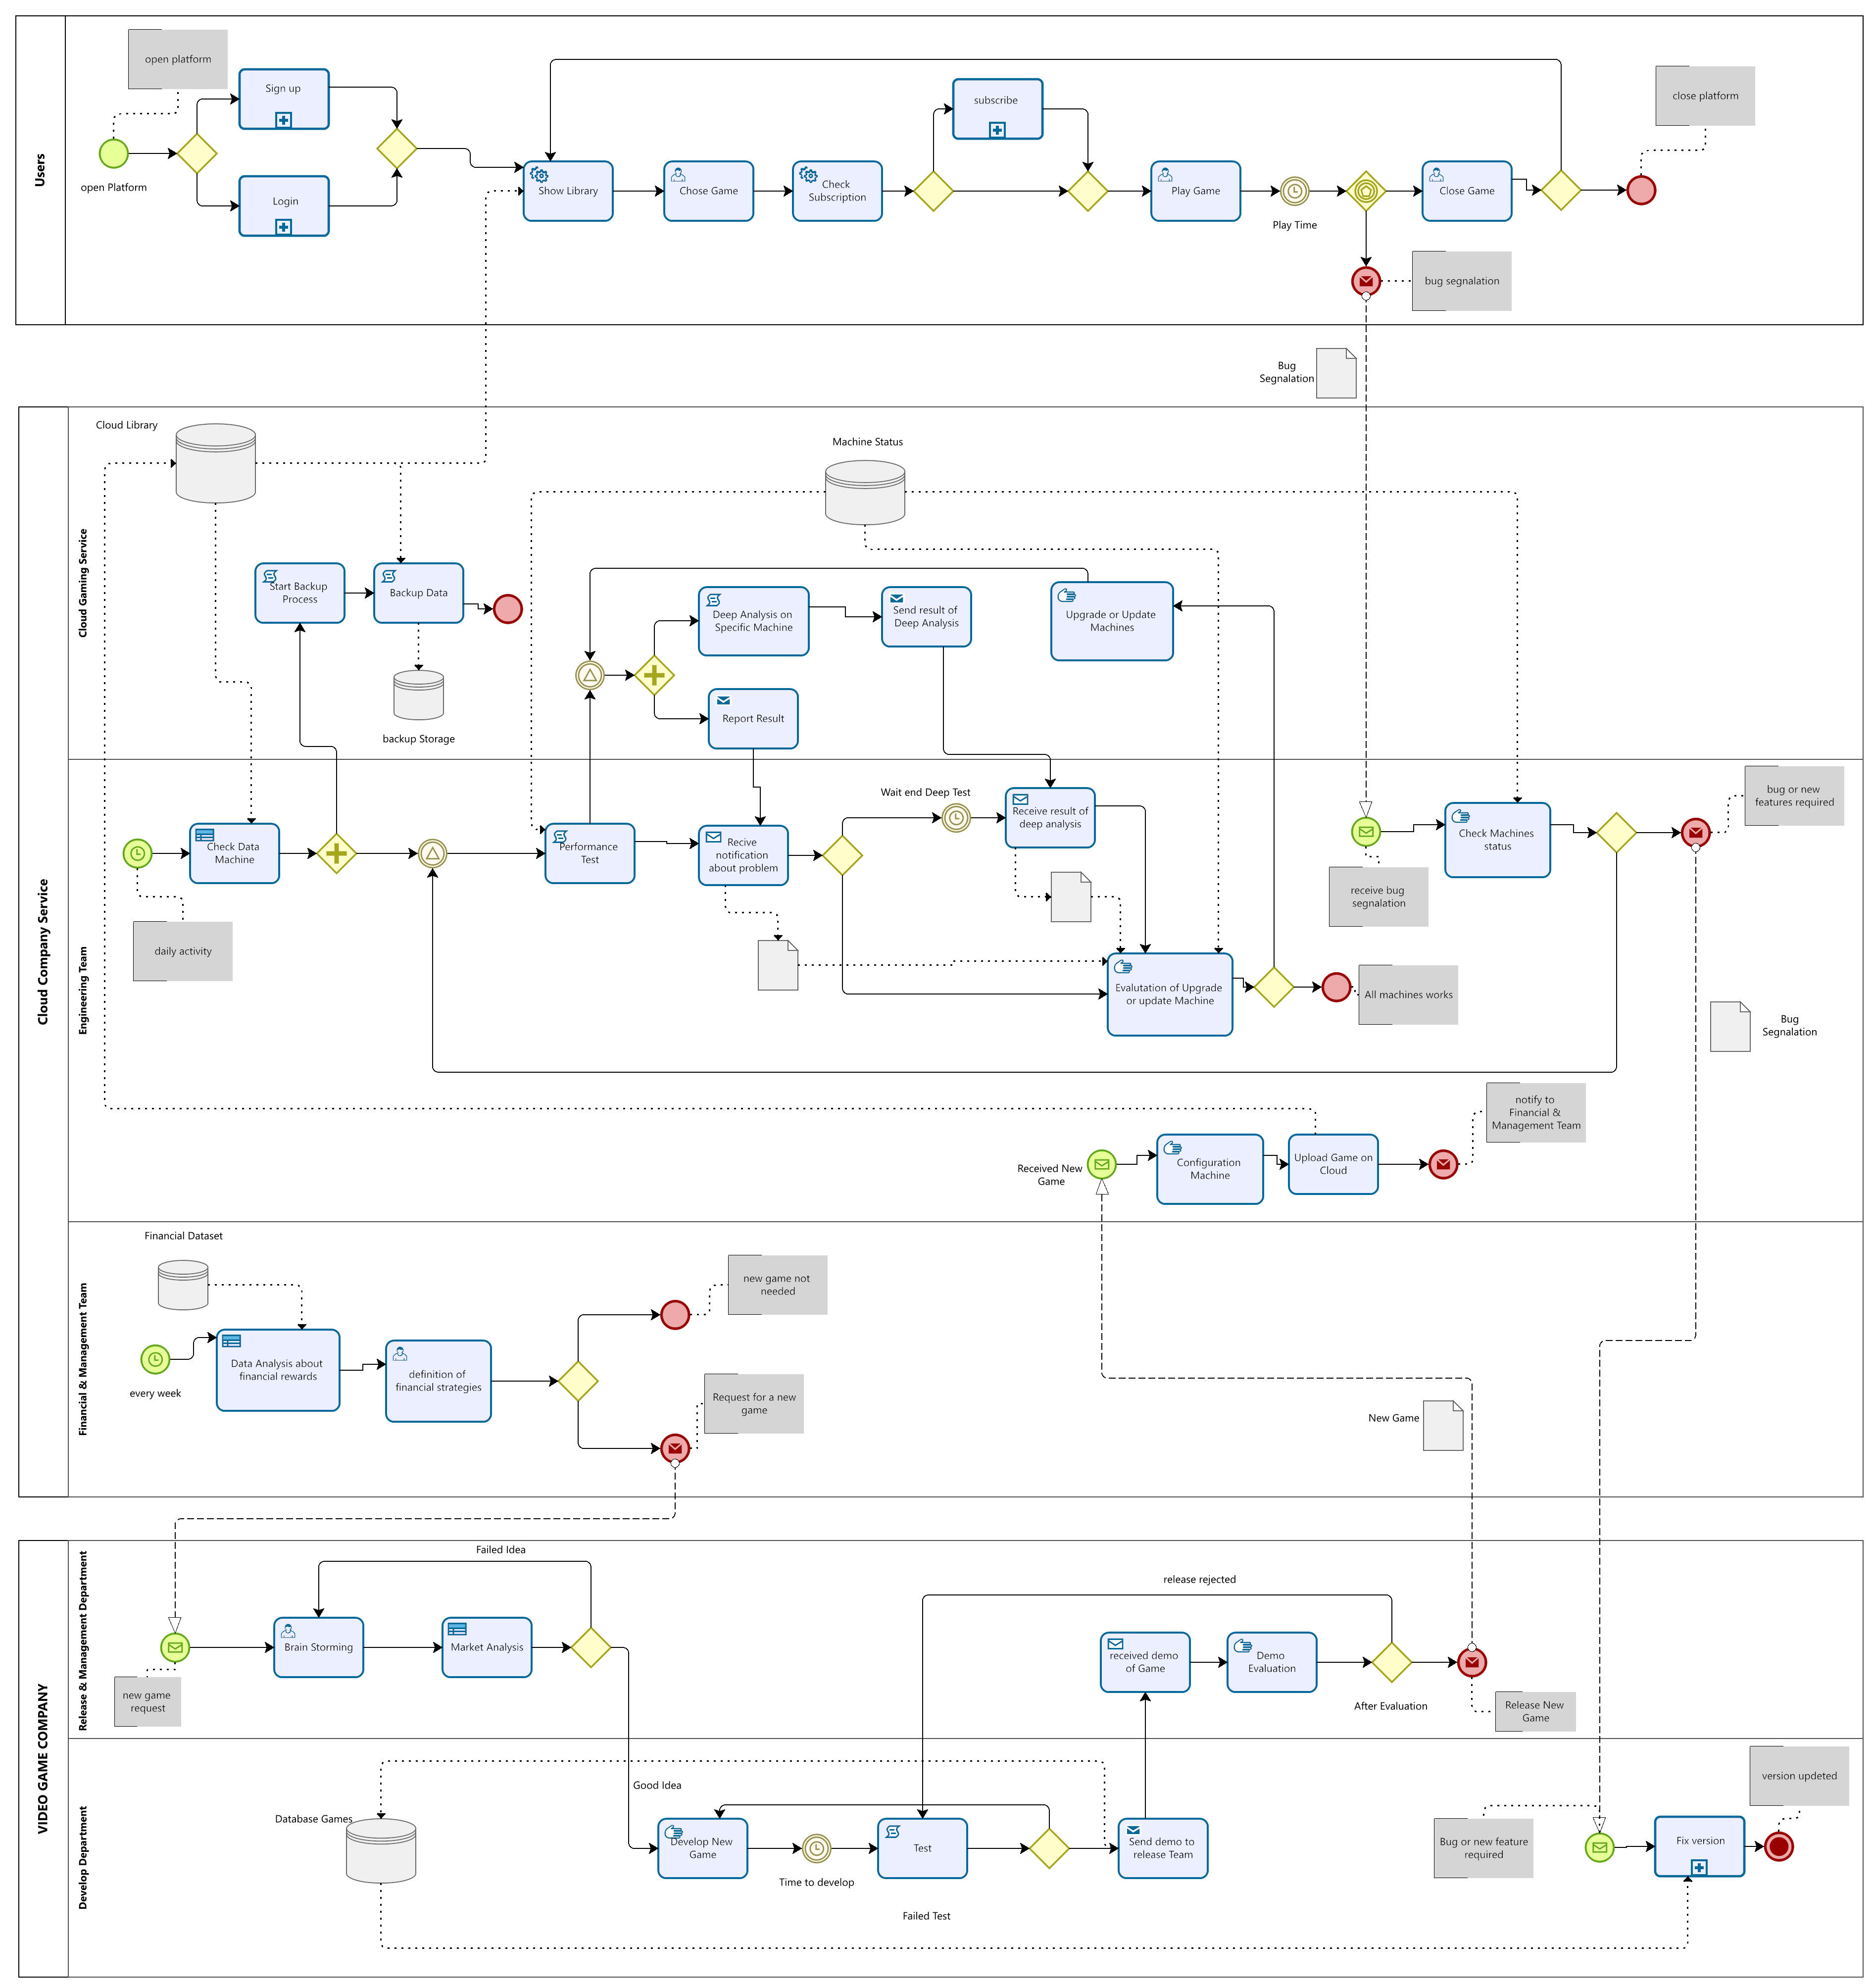
\includegraphics[scale=0.15]{Full_BPMN}
\caption{Full BPMN Diagram}
\label{FULL BPMN}
\end{figure} 
%
%
\section{The Users}
\begin{figure}[H]
 \centering
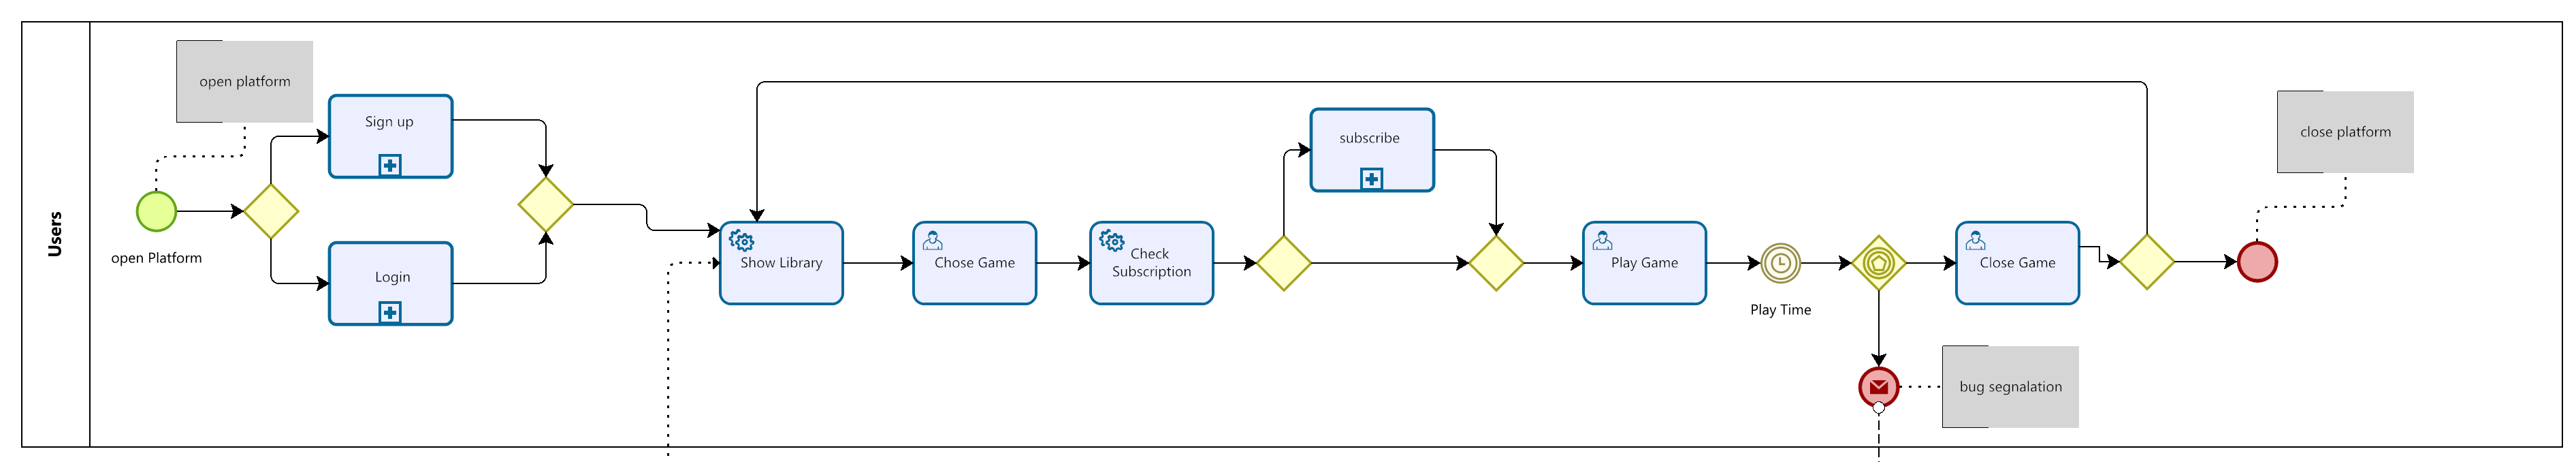
\includegraphics[scale=0.16]{user_BPMN}
\caption{Users BPMN Diagram}
\label{Users BPMN}
\end{figure} 

\subsection{Sub Process - Login }
\begin{figure}[H]
 \centering
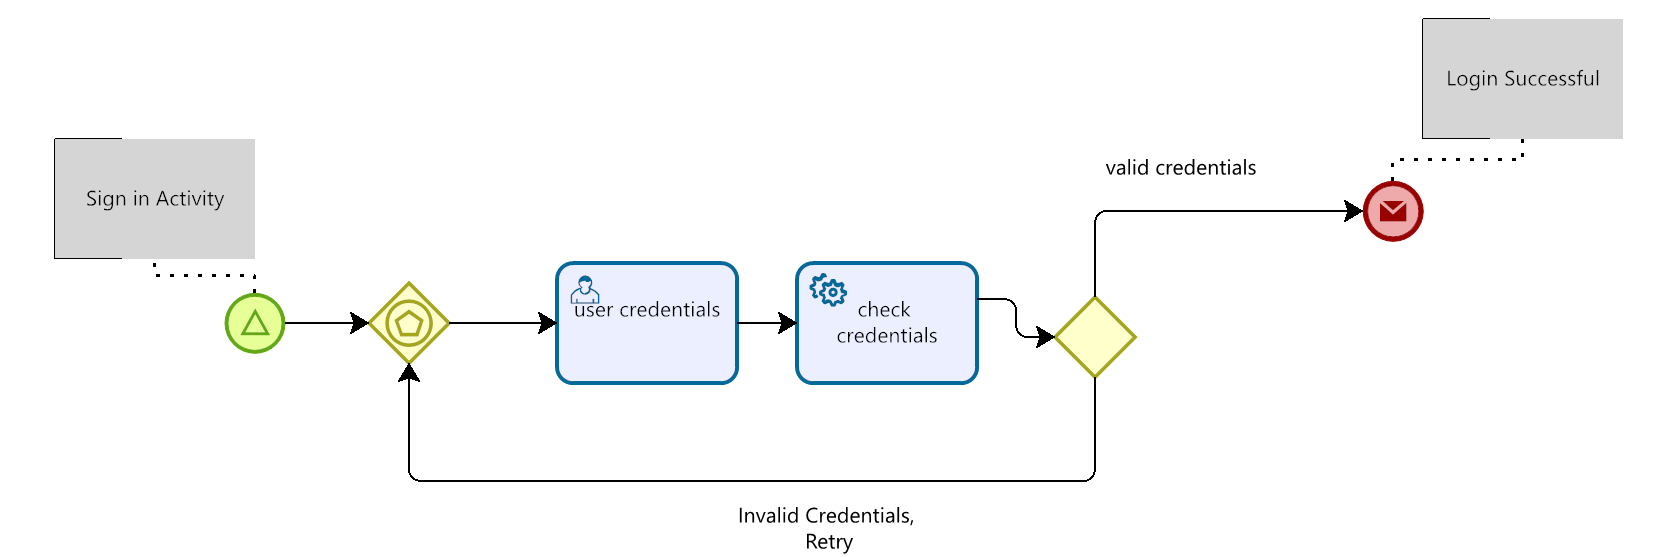
\includegraphics[scale=0.35]{login_BPMN}
\caption{Sub Process - Login BPMN Diagram}
\label{Login BPMN}

\end{figure} 

\subsection{Sub Process - Register }
\begin{figure}[H]
 \centering
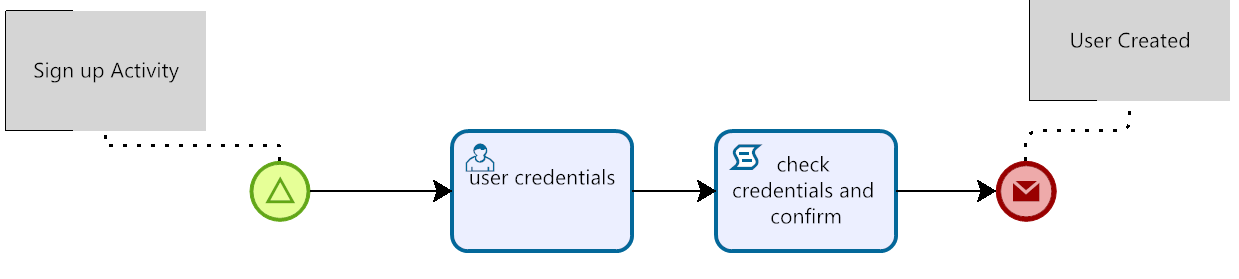
\includegraphics[scale=0.35]{signup_BPMN}
\caption{Sub Process - Sign up BPMN Diagram}
\label{Signup BPMN}
\end{figure} 

\subsection{Sub Process - Subscription }
\begin{figure}[H]
 \centering
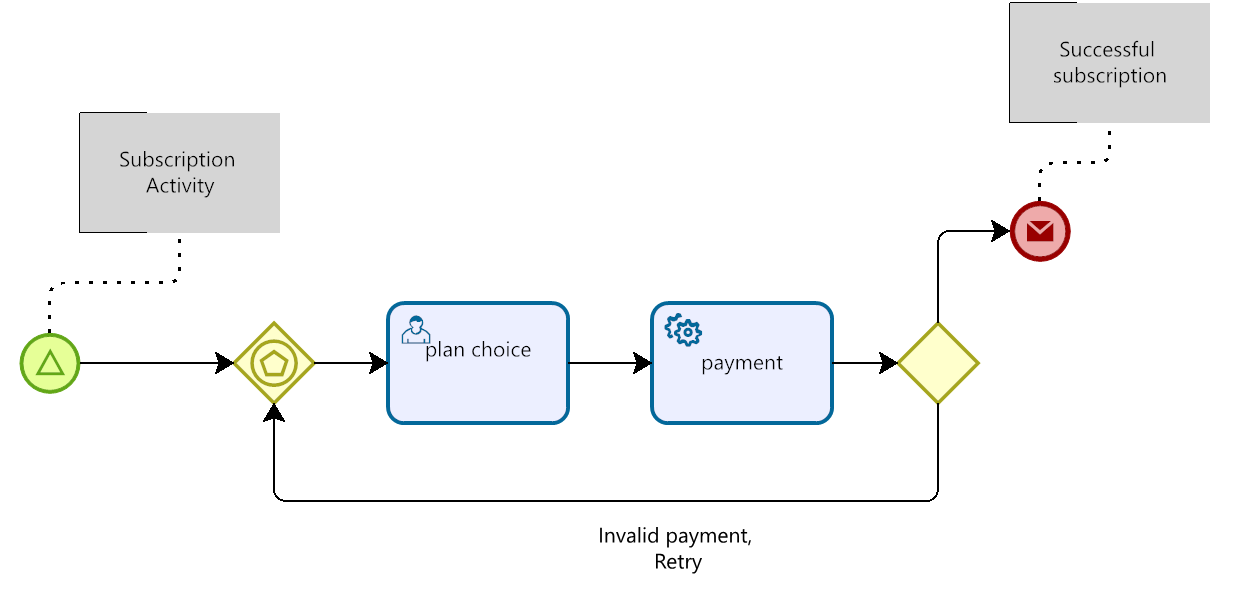
\includegraphics[scale=0.35]{subscription_BPMN}
\caption{Sub Process - Subscription BPMN Diagram}
\label{Subscription BPMN}
\end{figure} 

\section{The Cloud Computing service }
\begin{figure}[H]
 \centering
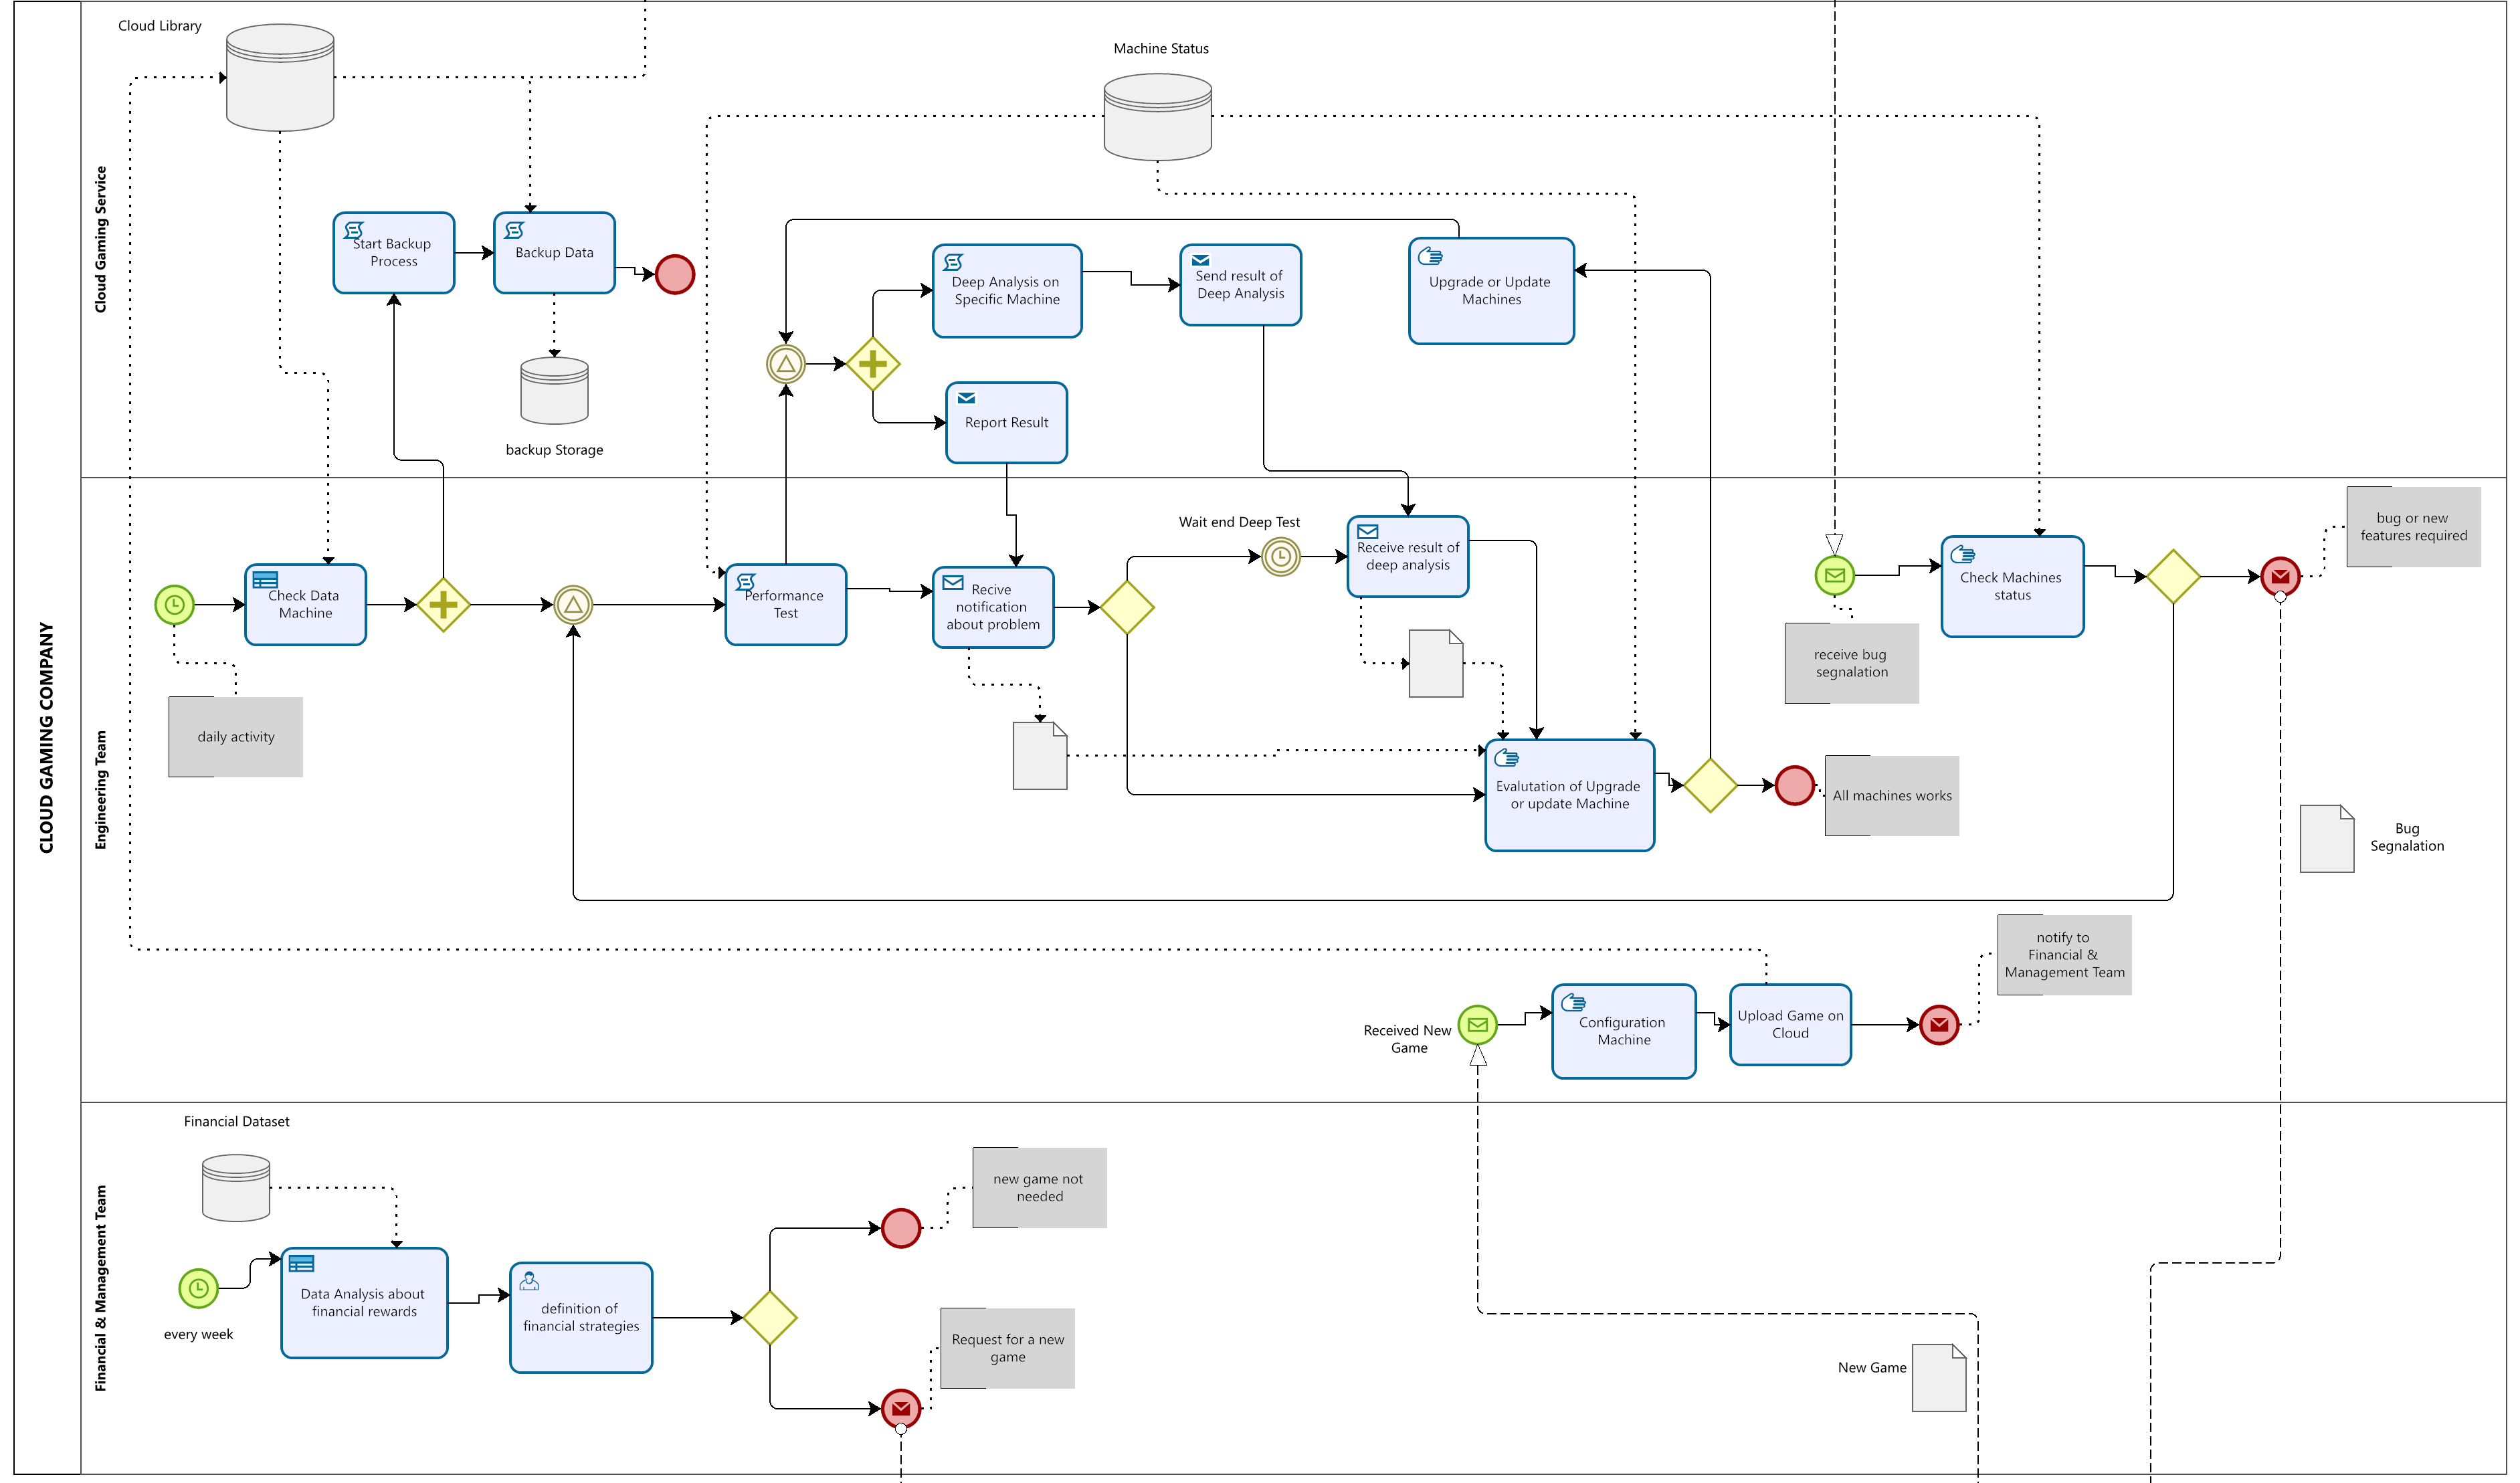
\includegraphics[scale=0.15]{cloud_BPMN}
\caption{Cloud Computing Service BPMN Diagram}
\label{Cloud BPMN}

\end{figure}



\section{The video game company  }
\begin{figure}[H]
 \centering
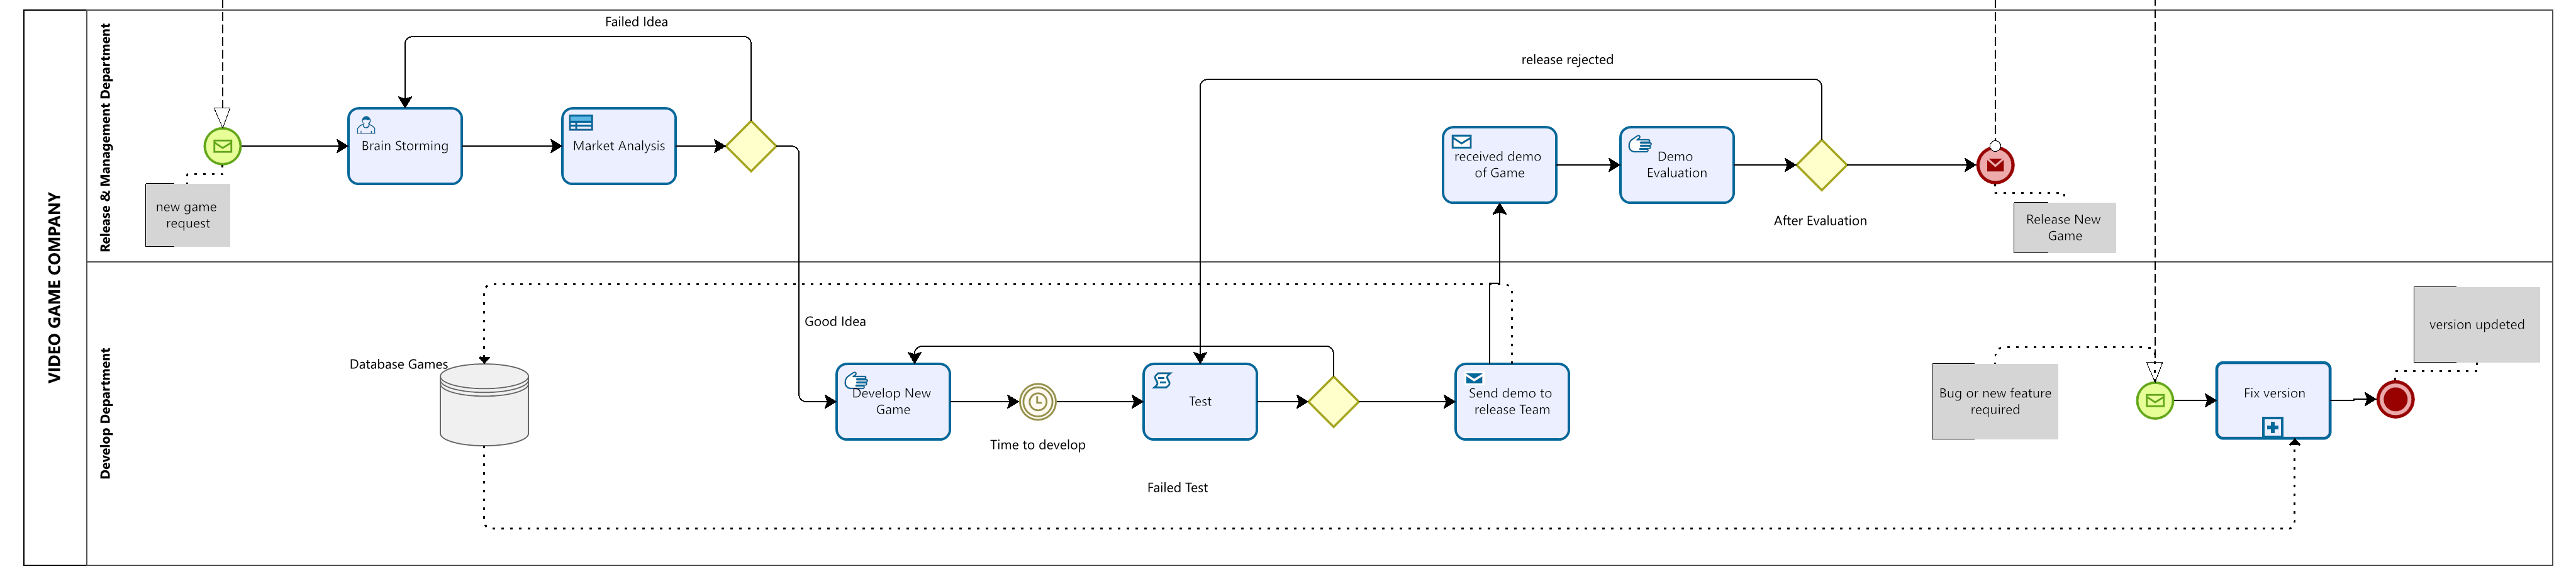
\includegraphics[scale=0.15]{videogame_BPMN}
\caption{Video Game Company BPMN Diagram}
\label{VideoGame BPMN}
\end{figure} 

\subsection{Sub Process - Fix Version }
\begin{figure}[H]
 \centering
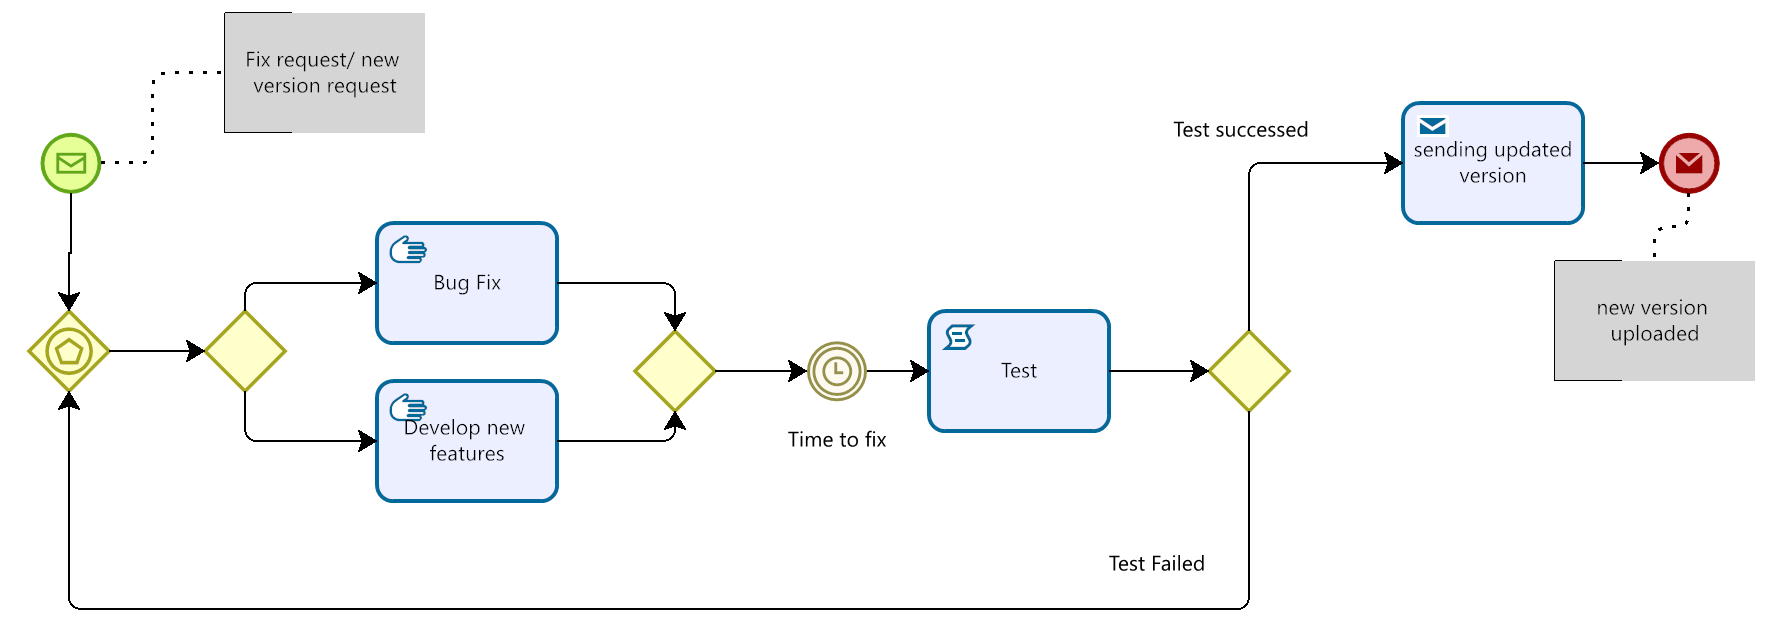
\includegraphics[scale=0.35]{developer_BPMN}
\caption{Sub Process - Fix Version BPMN Diagram}
\label{Fix Version BPMN}

\end{figure} 

\chapter{Value Model}
The Value Model describes what constitutes value in an organization, where organizations create value, how stakeholders exchange value, and, most importantly, how an organization can find new opportunities to create value.\\
A Value Model is basically a diagram designed to represent the exchange of services and payments
between different actors and/or market segments. In most cases there is no way to get
this diagram somehow, it has to be created from scratch.

\subsection{Structure of Value Model}
\begin{itemize}
\item{\textbf{Actor:} is an economically independent entity. It is represented by a square}
\item{\textbf{Value Exchange:} connects two Value Ports with each other. It is represented by lines}
\item{\textbf{Value Interface:} groups an input/output Value Ports. It is atomic.}
\item{\textbf{Value Ports:} is used by an actor to provide or request Value Objects to and from other
actors. It is an abstraction of internal business processes and can be an incoming input or output.}
\item{\textbf{Market Segment:} is a set of actors who assign same value to certain objects..}
\end{itemize}
%
%
\newpage
\section{Actor}
\paragraph*{Users}
\begin{itemize}
\item{\textbf{Users:} Market segment actor using the cloud platform in return for payment.
Users can play on the platform any game made available by the cloud computing service.} 
%
\end{itemize}
%
%
\paragraph*{Cloud Gaming Company}
\begin{itemize}
\item{\textbf{Cloud Gaming Service:} Actor referring to the cloud gaming platform.
This platform contains the games uploaded by the engineering team. This team is also responsible for the maintenance of the platform. Users can register and use the platform. } 
%
\item{\textbf{Engineering Team:}  Actor referring to the engineering team.
The engineers team works for the cloud gaming service, they monitor the platform, perform maintenance, update and add new content, and operate in case there are bugs on the service. } 
%
\item{\textbf{Financial \& Management Team:}  Actor referring to the Financial \& Management team.
This team is in charge of checking the performance of the platform in terms of economics, evaluating data, and requesting new content from the Video Game company. } 
%
\end{itemize}
%
%
\paragraph*{Video Game Company}
\begin{itemize}
\item{\textbf{Develop Department:} Actor who is part of the video game company.
His job is to release new games defined by the Release \& Management department. It is also in charge of updating existing games and making bug fixes when they are reported } 
%
\item{\textbf{Release \& Management Department:}  Actor who is part of the video game company.
His job is to communicate with the Financial \& Management Team to define new games and analyze their cost. In addition to the business aspect, he is in charge of releasing the game as a result of the request from the cloud gaming service to have a new content on the platforms.
} 
\end{itemize}
\section{Value Diagram}

\begin{figure}[H]
 \centering
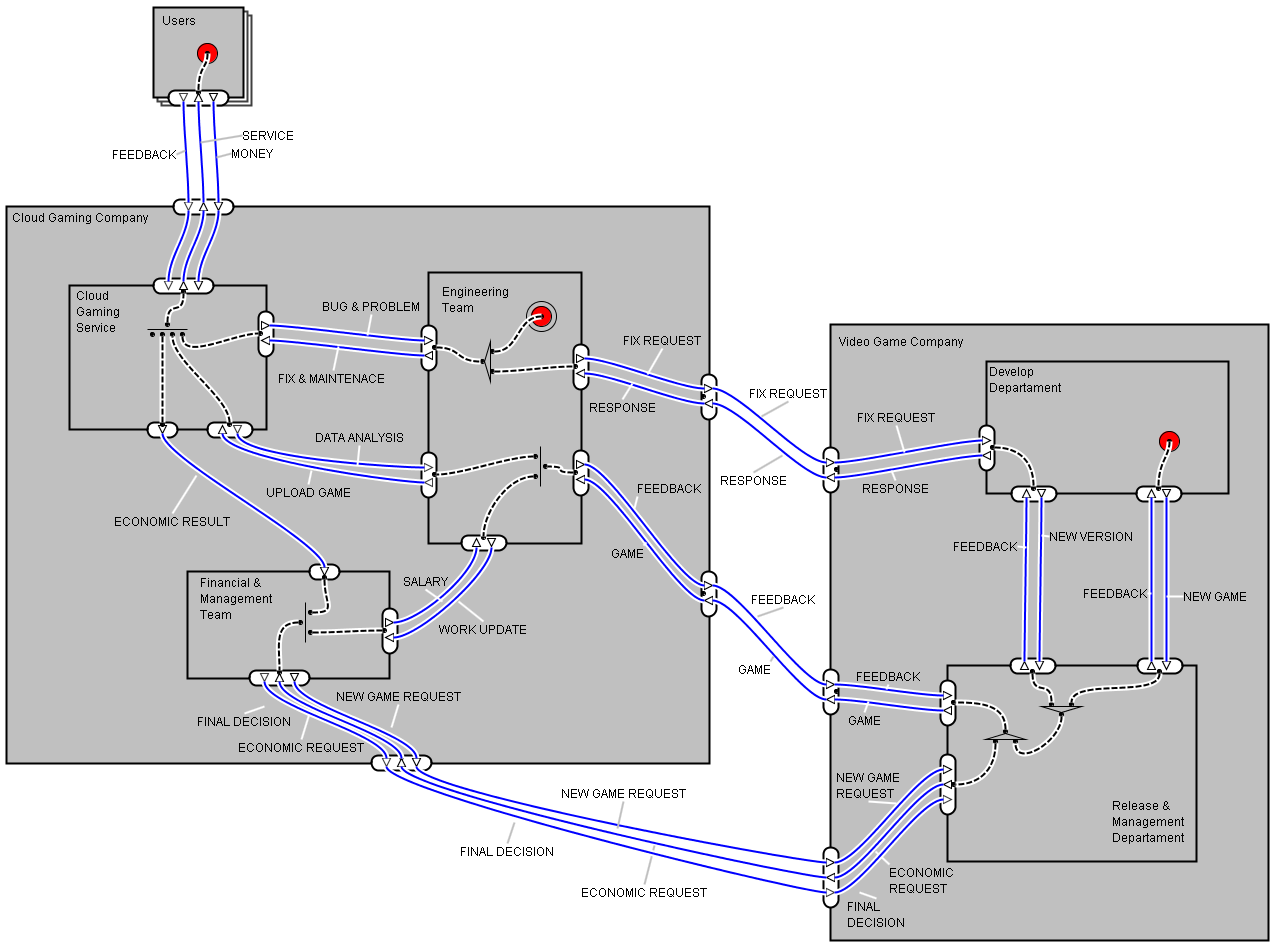
\includegraphics[scale=0.45]{value_model}
\caption{Value Diagram}
\label{Value Diagramn }
\end{figure} 

\chapter{Business Evaluation}
In this part of the project, assumptions were made about what the evaluation criteria of the above-mentioned business might be. \\
In fact, it was intended to hypothesize some factors such as Critical Successor Factors, Key goal Indicators, and Key performace Inficators. \\
All these factors were calculated hypothetically as we do not have any real data related to a cloud gaming service. \\
The purpose of this section is to show a pontential analysis that could be applied in a real-world context. 
\section{Critical Successor Factors (CSF)}
Critical success factors (CSFs) are critical factors or activities that can evaluate the success of the company. In our case study, we can denote as CSFs:
\begin{itemize}
\item{\textbf{Number of subscribed users:} the higher the number of subscribed users, the higher the revenue of the cloud service and consequently the more budget is available to buy and have new games produced }
\item{\textbf{Number of hours per user on the platform:} the more a user uses the platform the more it means they are satisfied, this could ensure a prolonged subscription over time.  }
\item{\textbf{Number of shares by the user:} for example, sharing on social networks, which could lead more users to subscribe.}
\item{\textbf{Number of platform disservices:} the lower the number of reports on platform operation, the higher the level of satisfaction increases}
\end{itemize}
\newpage
\section{Key Goal Indicators}
Key Goal Indicators (KGI) define the metrics to check whether the company's goal has been achieved. 
For example, they are useful goals for quantifying business progress. In our case we can define:
\begin{itemize}
\item{\textbf{New subscribers:} the steady increase in the number of users subscribing to the service ensures that the company can grow. }
\item{\textbf{Growth in service use:} users are using the platform more often ensures continued service growth.}
\item{\textbf{Increased sharing by users:} Increase users' sharing of content on social platforms to gain more visibility and active users } 
\item{\textbf{Reduce disservices on platform:} the lower the number of reports on platform operation, the higher the level of satisfaction increases}
\end{itemize}
\section{Key Performance Indicators}
Key Performance Indicators (KPIs) are an index that express what you want to
achieve by when. They are the quantifiable, outcome-based statements you’ll use to measure if
you’re on track to meet your goals or objectives.
KPIs are used to measure the results achieved by the organization.\\ In the case we can define:
\begin{itemize}
\item{\textbf{Rate of new subscribed users:} Number of new users who subscribe to the system in a defined time ( i.e. daily, monthly... ) }
\item{\textbf{Average time on the platform:} Average time spent within the platform by users  }
\item{\textbf{Average of monthly accesses:} Average of monthly accesses by a subscribers users on the platform  }
\item{\textbf{Number of monthly shares by the users:} Number of sharing on social networks, which could lead more users to subscribe.}
\item{\textbf{Number of platform disservices:} The value is the number of daily reports made by users.}

\end{itemize}

\section{KPI in Practice}

\begin{figure}[H]
 \centering
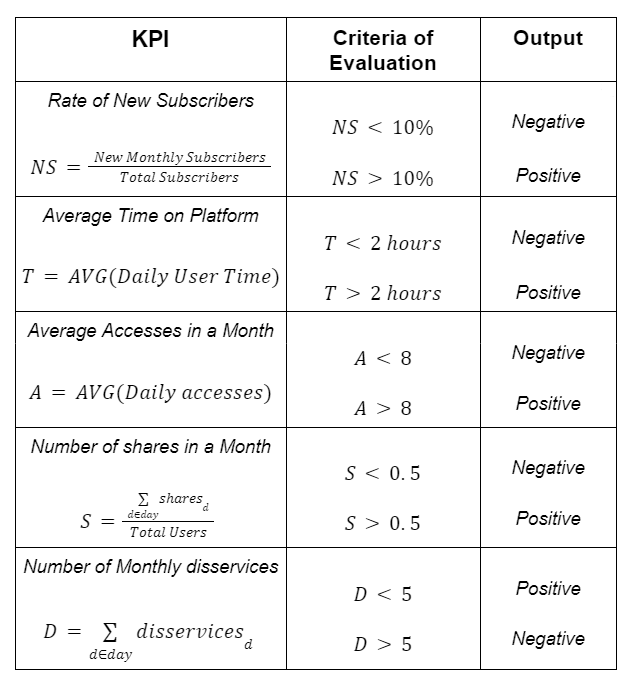
\includegraphics[scale=0.8]{KPI}
\caption{KPI evaluation}
\label{KPi }
\end{figure} 

\chapter{Conclusion}
In conclusion, this new technology will evolve in the future and make it more accessible to play from any device without the need for high performance. 
In this project, we wanted to represent a model of how the company would operate in order to identify the factors necessary for growth.\\
Although the entire drafting was based on a hypothetical structure of a cloud gaming service company it was possible to represent in detail all process steps and business-side evaluation criteria. In particular, the BPMN diagram and the Value Model diagram made it possible to show the unfolding of the process and to illustrate in a simple and intuitive way all the stages of developing and enjoying a video game on a cloud platform.\\
Through CSFs, KGIs the KPIs it is possible to evaluate better strategies to achieve greater profits and reach as many people as possible.\\\\
%
As mentioned above unfortunately there was no real data available especially concerning the evaluation criteria that each company uses to define a business strategy, nevertheless it was possible to simulate a hypothetical case study in which a real company that uses this type of service could be placed
\end{document}


 
